%%%%%%%%%%%%%%%%%%%%%%%%%%%%%%%%%%%%%%%%%%%%%%%%%%%%%%%%%%%%%%%%%%%%%%%%
%%%%%                                                              %%%%%
%%%%% Chapter 4: Identifying SMURF-seq fragment boundaries         %%%%%
%%%%%                                                              %%%%%
%%%%%%%%%%%%%%%%%%%%%%%%%%%%%%%%%%%%%%%%%%%%%%%%%%%%%%%%%%%%%%%%%%%%%%%%
\chapter{Identifying fragment boundaries on a SMURF-seq read}
\label{ch4}

%%%%%%%%%%%%%%%%%%%%%%%%%%%%%%%%%%%%%%%%%%%%%%%%%%%%%%%%%%%%%%%%%%%%%%%%
%%%%%%%%%%%%%%%%%%%%%%%%%%%%%%%%%%%%%%%%%%%%%%%%%%%%%%%%%%%%%%%%%%%%%%%%
%%%%%%%%%%%%%%%%%%%%%%%%%%%%%%%%%%%%%%%%%%%%%%%%%%%%%%%%%%%%%%%%%%%%%%%%
\section{Motivation}
%% Sequencing tech and mapping methods
New sequencing methods motivate development of new algorithms for
mapping and analysis of sequences generated using these methods. A few
significant developments include BLAST \citep{altschul1990basic} and
FASTA \citep{pearson1988improved} motivated by database searches with the
advent of Sanger sequencing, BWA \citep{li2009fast} and Bowtie
\citep{langmead2009ultrafast} inspired by high-throughput short-read
sequencing, and BLASR \citep{chaisson2012mapping} by single-molecule
long-read sequencing.
%% SMURF-seq
SMURF-seq has enabled efficient short-read sequencing for read-counting
applications on portable long-read machines.  However, efficient methods
tailored for mapping SMURF-seq reads are still lacking; Especially as
SMURF-seq protocol evolves and the fragments become shorter, and thus,
making the mapping process challenging in terms of identifying accurate
fragment locations and boundaries.

%% current SMURF-seq
As currently implemented, SMURF-seq protocol uses a single restriction
enzyme (SaqAI) to fragment DNA molecules to $\sim$150 bp. However,
depending on the downstream application, the fragment lengths need to be
just long enough to ensure unique mappability to a sufficient fraction
of the genome.
%% making fragments shorter
Fragments could be made shorter using methods discussed in section
\ref{}.  As an example, for copy-number profiling (at low
resolutions, as used for tumor samples) the fragment lengths could be as
short as 40 bp.

%% current barriers and how to remove them
We used BWA-MEM \citep{li2013aligning} to align SMURF-seq reads generated
with the current protocol, which consists of fragments that are
typically over 100 bp. Though not designed to align SMURF-seq reads,
BWA-MEM is designed for split read alignment, and it works sufficiently
well at these fragment lengths.  SMURF-seq reads can also be aligned
with other mapping tools capable of split-read alignment such as
Minimap2 \citep{li2018minimap2} and LAST \citep{kielbasa2011adaptive}.
However, all of these tools are either designed for aligning short reads
with low sequencing error or long reads with high sequencing error.

% Challenges as the fragments get shorter
Aligning SMURF-seq reads, especially as the fragments get shorter,
would differ from these tools in the following aspects: (1) A seeding
approach designed for short fragments sequenced with a high error-rate.
(2) An approach to estimate the number of fragments on a SMURF-seq read
and determine the optimal fragment boundaries.

% Seeding
The initial step of a typical alignment tool, called seeding, is to find
candidate locations of a read on the reference genome, and limit the
downstream steps to these locations.
%
This is usually using a hash table based data structure to find exact
matches \citep{altschul1990basic,altschul1997gapped,kent2002blat} or
non-contiguous exact matches \citep{ma2002patternhunter,chen2009perm},
or by using a suffix tree based data structure
\citep{kurtz2004versatile,langmead2009ultrafast,li2009fast,
li2010fast,li2013aligning}.
%
The choice of data structure and parameters such as the length of the
match, number of matches, etc. are determined by several factors such
as the read length and the error profile of the underlying sequencing
technology.
%
For example, the optimal seeds parameters for expressed sequence tags
and whole genome sequencing (prior to short-read high-throughput
sequencing) was determined in BLAT \citep{kent2002blat}, similarly for
low-error rate short-reads in RazerS \citep{weese2009razers}, and
high-error rate long-reads in BLASR \citep{chaisson2012mapping}.
%
The fragments could be as short as 40 bp in a SMURF-seq read, and
aligning these reads requires identifying candidate locations for these
fragments in the presence of the characteristic error profile of
nanopore machines.


% Importance of having accurate fragment boundaries
The significance of having accurate fragment boundaries is understood by
looking at the fraction of the genome that is uniquely mappable. For the
human reference genome (hg19), when allowing no mismatches or indels,
the fraction of the genome that is uniquely mappable reduces by 0.06\%
when going from 150 to 145 bp, whereas it reduces by 2.02\% when going
from 40bp to 35bp (Fig.~\ref{dzones}).
% how it affects SMURF-seq read
Thus, as the fragments get shorter, the probability of a fragment that
originated from a unique location on the genome to misalign to an
ambiguous location or vice-versa increases.
% reads with errors
% TODO: Improve sentence below
Further, as sequencing errors are considered the difference in unique
mappability due to having inaccurate fragment boundaries is likely to
increase.
%
Thus, as the fragments become shorter, having accurate fragment
boundaries would improve the sensitivity of aligning SMURF-seq reads.

\begin{figure}[t!]
\centering
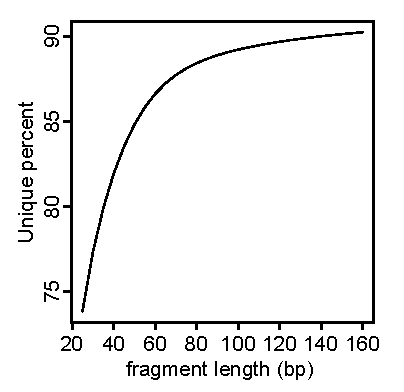
\includegraphics{ch4_fig1.pdf}
\caption[Uniquely mappable fraction of the genome decreases fragment
  length]{
  The fraction of genome that is uniquely mappable decreases with
  fragment length.}
\label{dzones}
\end{figure}


%% How will our method remove the current barrier
Although both seeding and determining the accurate fragmentation is
crucial to align a SMURF-seq read, in this study we focus only on the
second. To this end, we define the fragment identification problem for
identifying the number of fragments and the fragment boundaries on a
SMURF-seq read.  We approach the fragment identification problem by
defining a score function for aligning a SMURF-seq read, study the null
score distribution of aligning reads and reference generated at random,
and estimate the number of fragments in a SMURF-seq read by comparing
its alignment score with the null distribution for all possible
fragmentations of a read.  Then we show the accuracy of our method using
from simulated genomes and SMURF-seq reads. Further, we empirically show
that this method could also be used with a general score function.

%%%%% How will this improve scientific capacity and knowledge




%%%%%%%%%%%%%%%%%%%%%%%%%%%%%%%%%%%%%%%%%%%%%%%%%%%%%%%%%%%%%%%%%%%%%%%%
%%%%%%%%%%%%%%%%%%%%%%%%%%%%%%%%%%%%%%%%%%%%%%%%%%%%%%%%%%%%%%%%%%%%%%%%
%%%%%%%%%%%%%%%%%%%%%%%%%%%%%%%%%%%%%%%%%%%%%%%%%%%%%%%%%%%%%%%%%%%%%%%%
\section{Background}
\label{ch4_background}
In the early days of DNA sequencing, as the number of nucleotides
sequenced grew, comparison of DNA sequences became an indispensable tool
to a biologist.
%
DNA sequence comparison can be broadly classified into global alignment
\citep{needleman1970general} and local alignment
\citep{smith1981identification}. A global alignment seeks an optimal
alignment between two sequences such that each base of one sequence is
aligned to each base of the other sequences. On the other hand, a local
alignment seeks an optimal alignment between any subsequences of the
sequences being compared.

Comparison of two sequences, even unrelated or random sequences, always
produces an optimal alignment. This motivated the development of
approaches to differentiate a ``meaningful'' alignment from alignment of
unrelated sequences. These methods determine the significance of an
alignment by comparing the alignment score with a null distribution of
alignment scores of unrelated sequences. Determining the appropriate null
distribution was the subject of an enormous amount of research, some of
which are summarized below.

%% Simulation studies
In the context of local alignment, at the time of the initial studies on
the score distribution of unrelated sequences, mathematical tools to
understand the null distributions were still lacking, and these studies
relied on empirical distributions generated from aligning unrelated
sequences.
%%
In \citep{smith1985statistical}, it is shown that the similarity score is
proportional to the logarithm of the length of the sequences being
compared, and the standard deviation is independent of the sequence
length. The significance of an alignment was determined from the number
of standard deviations over mean of the alignment score.
%% Dependence on sequence properties
These studies \citep{lipman1984statistical} also highlight that the
statistical properties \citep{smith1983statistical}, such as nucleotide
frequencies or codon usage, of the sequences affect the distribution of
the alignment scores.  Generating a null distribution from an incorrect
model could lead to an alignment of unrelated sequences being dubiously
declared significant. Several methods are available to generate random
sequences preserving these statistical properties
\citep{fitch1983random,altschul1985significance}.

%% Mike's approach: coin tossing
Erdos and Renyi \citep{erdos1975length} presented results for the length
of the longest headrun in a the first $n$ tosses of a biased coin.  The
length of the longest headrun in coin tosses is equivalent to the number
of matches between two DNA sequences when shifts in the starting and
ending positions of the sequences are not allowed, with the probability
of head equal to the probability of match between letters of the DNA
alphabet.
% coin tossing with shifts and fixed mismatches.
In \citep{arratia1985erdos}, this is generalized to matches between DNA
sequences, while allowing shifts. These results indicate that allowing
shifts doubles the length of the longest headrun. Results for the
longest headrun allowing for up to $k$ mismatches and sequences
generated from a Markov chain are also considered.
% EVD approximation
In \citep{arratia1986extreme,gordon1986extreme} the distribution of the
longest matches is shown to a have an extreme value distribution with
mean that is proportional to the logarithm of the sequences lengths and
variance independent of sequence length. Here, when considering only
matches, the asymptotic extreme value distribution is shown by
considering a maximum of geometric distributions, and when mismatches
are allowed, it is shown by considering a maximum of negative binomial
distributions.
% poisson approximation
An alternate approach is a Poisson approximation for the distribution of
the longest match \citep{arratia1989erdos}.

%% Dembo and Karlin's approach
An crucial aspect of in aligning nucleic acid and protein sequences is
using the appropriate score function. For example, PAM and Dayoff
matrices is used for protein sequences \citep{}, and xxx is used for DNA
sequences \citep{}.  The score function used alters the score of the
aligned sequences and thus the alignment score distribution of unaligned
sequences.
% Headrun approach does not consider score function
However, the approach based on the length of the headruns does not
consider the score function used for an alignment.
%
In \citep{}, it is shown that the score distribution of aligning
unrelated sequences for any score function (that has at least one
positive score and the expected score is negative) has the form of an
extreme value distribution, and and explicit formulas that its parameters
are provided.
% distribution of letters, and log-odds ratio



%% alignment allowing gaps

%% BLAST

%% Profile alignment

%% Global alignment score distribution

%% Differneces between these and the k=1 frag id problem




%% local alignment
% The local alignment score distribution has been studied extensively,
% especially in the context of BLAST score statistics
% \citep{altschul1990basic,altschul199627}.  The distribution of the local
% alignment score is well approximated by the extreme value distribution
% (EVD) \citep{karlin1990methods,
% karlin1990statistical,dembo1994limit,dembo1991strong}.

% It has also been shown that the distribution of the maximum score
% obtained when a profile sequence is aligned to all possible positions of
% a random sequence has a limiting extreme value distribution
% \citep{goldstein1994approximations}.


%%%%%%%%%%%%%%%%%%%%%%%%%%%%%%%%%%%%%%%%%%%%%%%%%%%%%%%%%%%%%%%%%%%%%%%%
%%%%%%%%%%%%%%%%%%%%%%%%%%%%%%%%%%%%%%%%%%%%%%%%%%%%%%%%%%%%%%%%%%%%%%%%
%%%%%%%%%%%%%%%%%%%%%%%%%%%%%%%%%%%%%%%%%%%%%%%%%%%%%%%%%%%%%%%%%%%%%%%%
\section{Fragment Identification problem}
%% string properties
Let $\Sigma$ be an alphabet. A string $X$ is a sequence of letters $a_0
a_1 \dots a_{n-1}$, where $a_i \in \Sigma$; $|X|$ denotes the length of
the string $X$; and $X[i \dots j] = a_i \dots a_{j-1}$ is a substring of
$X$.

%% reference string
The reference string $T$ is generated from the DNA alphabet $\Sigma =
\{A, T, G, C\}$, with $|T| = n$.
%% SMURF-seq string
A SMURF-seq read $S$ is generated by concatenating substrings (called
fragments) of $T$, with no information available \textit{a priori} about
the number, length, orientation (forward or reverse-complement), and the
position on $T$ of these fragments.  Further, $S$ contains sequencing
errors with a rate $\rho$. Let $|S| = m$ and $m \ll n$.

%% fragment set
A fragment set $P$ is an set of start locations of fragments on $S$. $P
\subset \{0 \dots m-1\}$ and $|P| = k$, with the rule that $0$ is in $P$
always.
%%
By convention we consider the set $P$ to be ordered such that if $i < j$
then $P_i < P_j$.
%%
For a fragment set $P$, $\sum_{i = 1}^{k} P_{i+1} - P_i = m$ and we say
that the $i^{\text{th}}$ of $S$ is the substring $S[P_i \dots P_{i+1}]$,
with $P_{k+1} = m$.

%% fragment identification problem
For a given $T$ and $S$, the fragment identification problem is to
determine the elements of the fragment set $P$ such that it corresponds
to the start locations of fragments contained in $S$.



%%%%%%%%%%%%%%%%%%%%%%%%%%%%%%%%%%%%%%%%%%%%%%%%%%%%%%%%%%%%%%%%%%%%%%%%
%%%%%%%%%%%%%%%%%%%%%%%%%%%%%%%%%%%%%%%%%%%%%%%%%%%%%%%%%%%%%%%%%%%%%%%%
%%%%%%%%%%%%%%%%%%%%%%%%%%%%%%%%%%%%%%%%%%%%%%%%%%%%%%%%%%%%%%%%%%%%%%%%
\section{Approach to the fragment identification problem}
We approach the fragment identification problem by defining a score
function as follows:
%% score function
For a given fragment set $P$, we define the score of aligning $S$ to $T$
as: \[score_T(S,P) = \sum_{i=1}^{k} \max\{score(T[u \dots v], S[P_i
\dots P_{i+1}]): 0 \leq u < v \leq n\}.\]
%
This allows us to consider the fragment identification problem as two
inter-related problems: (1) Determining $k$, the size of the fragment
set, and (2) given $k$, determining the elements of $P$ such that
$score_T(S, P)$ is maximized.

%% Any k gives a score. Highest score does not correspond to the opt.
By the score function defined above, to determine the elements of the
fragment set $P$, requires the knowledge of the number of fragments $k$
and this is not known \textit{a priori}. Further, the $k$ that maximizes
the score function would almost never correspond to the optimal fragment
set. As an example, taking $k=m-1$ which corresponds to taking each base
as a fragment would maximize the score, however, this is a non-sensical
alignment.

%% Outline of our statistical approach.
We propose to estimate the number of fragments $k$ by aligning a read
to the reference genome with different $k$. For each of these
fragmentations, we determine the p-value by comparing the alignment
score with the null distribution generated from aligning reads generated
at random to a reference genome generated at random. Finally, we choose
the fragmentation with lowest p-value as the optimal fragmentation.

%% Differences with the local alignment approach We are interested in
%% opt frags, and not significant alignment
The fragment identification problem differs from the alignment problems
described in section \ref{ch4_background} in a crucial manner. For the
fragment identification problem we have the reference genome, and it is
assumed that the reads always arise from this genome; the score
distribution of sequences generated at random is used to determine the
optimal number of fragments on a SMURF-seq read. Whereas in the context
of local alignment the score distribution of aligning random reads are
used to determine a ``meaningful'' alignment by comparing the alignment
score of sequences with the random null distribution.



%%%%%%%%%%%%%%%%%%%%%%%%%%%%%%%%%%%%%%%%%%%%%%%%%%%%%%%%%%%%%%%%%%%%%%%%
%%%%%%%%%%%%%%%%%%%%%%%%%%%%%%%%%%%%%%%%%%%%%%%%%%%%%%%%%%%%%%%%%%%%%%%%
%%%%%%%%%%%%%%%%%%%%%%%%%%%%%%%%%%%%%%%%%%%%%%%%%%%%%%%%%%%%%%%%%%%%%%%%
\section{Aligning SMURF-seq reads and identifying fragment boundaries}

%% TODO: Need to change this
% why do we need this?
Having a score function for SMURF-seq reads enables a statistical
approach to estimate the number of fragments on a read. The proposed
method depends on an algorithm that can identify the optimal fragment
boundaries, given the number of fragments, such that the sum of the
alignment score of each fragment is maximized.

%%%%%%%%%%%%%%%%%%%%%%%%%%%%%%%%%%%%%%%%%%%%%%%%%%%%%%%%%%%%%%%%%%%%%%%%
\subsection{Fragment boundary identification under exact matching}
We first examine the fragment identification problem assuming the score
function requires exact matching
\[score(a,b)=
\begin{cases}
  1 & \text{if } a = b \\
  -\infty & \text{otherwise.}
\end{cases}\]
The fragment identification problem then becomes an exact matching
problem where the goal is to minimize the number of fragments such that
$score_T(P,S)$ is maximized.

A simple linear time solution to this problem can be obtained as
follows. First, we assume some data structure for $T$ has been
constructed in linear time and allows for longest prefix matches to be
computed in time proportional to the length of the query string. The
data structure could be a suffix tree \citep{mccreight1976space}, or a
more space efficient and a modern structure like an FM-index
\citep{ferragina2000opportunistic}. The principle of the algorithm can be
seen by starting at the beginning of $S$, and identifying the longest
prefix match of $S$ in $T$. Then retain $j$ as the first position of
where this longest prefix matches in $T$, and denote the first
mismatching position on $S$ as $i$. Repeat the procedure solving the
subproblem of fragment identification for $S[i\dots m]$. Repeating these
steps, the algorithm iteratively solves the longest prefix match
problems, retaining as $P_{i+1}$ the position of mismatch that
terminates matching during iteration $i$. The following pseudocode
describes the procedure.

\begin{algorithm}[H]
\caption{ExactFragmentMatching($T, S$):}
\begin{algorithmic}[1]
  \STATE $i \leftarrow 0$
  \WHILE{$i < m$}
    \STATE $P \leftarrow P\cup \{i\}$
    \STATE $i \leftarrow \text{longest-match-length}(S,i,T)$
  \ENDWHILE
  \RETURN $P$
\end{algorithmic}
\end{algorithm}

\textbf{Proof:} Consider an optimal solution to this problem, where the
identified fragment set $P_{\mathrm{opt}}$ has minimal size. To prove
the optimality of our algorithm we need to show that it finds the same
number of fragments as the optimal solution, i.e. $|P| =
|P_{\mathrm{opt}}|$.

The first iteration of the greedy algorithm will find the longest prefix
match. If the optimal solution has its first fragmentation ending before
$P_1$, i.e. $P_{\mathrm{opt1}} < P_1$. Then the longest match starting at
$P_{\mathrm{opt1}}$ will end at or before $P_2$, the end of the second
fragment found by the greedy algorithm. If it ends at $P_2$ then the
greedy algorithm has the same number of fragments as the optimal
solution so far. And it cannot end before $P_2$, because then the
optimal solution will have more fragments than found by the greedy
algorithm. Moreover, we cannot have $P_{\mathrm{opt1}} > P_1$ as this
would imply a longer prefix than found by the longest prefix match
exists. With this reasoning we can say that this greedy approach will
find just as little fragments as the optimal solution.

%%%%%%%%%%%%%%%%%%%%%%%%%%%%%%%%%%%%%%%%%%%%%%%%%%%%%%%%%%%%%%%%%%%%%%%%
\subsection{Fragment boundary identification allowing mismatches and indels}
Let $M$ denote a table with $m+1$ rows, $n+1$ columns and $k+1$
dimensions, where $k$ is the maximum number of fragments ($1 \leq k \leq
m$).  $\max_{0 \leq j \leq n}M(i,j,l)$ represents the best fragmentation
of $S[1 \dots i]$ with $l$ fragments. The entries of $M$ are computed as
follows:

\begin{algorithm}[H]
\caption{FragBoundaryIdentification$(T, S, k)$}
\begin{algorithmic}[1]
  \STATE $M(i,j,0) \leftarrow -\infty
          \text{ for all } 0 \leq i \leq m, 0 \leq j \leq n$
  \STATE $M(0,j,1) \leftarrow 0 \text{ for all } 0 \leq j \leq n$
  \STATE $M(i,0,1) \leftarrow M(i-1,0,1) + score(S[i], \_)
          \text{ for all } 0 \leq i \leq m$
  \STATE $M(l-1,j,l) \leftarrow -\infty \text{ for all } 2 \leq l \leq k,
          0 \leq j \leq n$
  \STATE $M(i,0,l) \leftarrow -\infty \text{ for all } 2 \leq l \leq k,
          l \leq i \leq m$
  \FOR {$l \leftarrow 1$ \TO $k$}
    \FOR {$i \leftarrow l$ \TO $m$}
      \FOR {$j \leftarrow 1$ \TO $n$}
        \STATE $M(i,j,l) \leftarrow \max
          \begin{cases}
            M(i-1,j-1,l) + score(S[i], T[j]) \\
            M(i-1,j,l) + score(S[i], \_) \\
            M(i,j-1,l) + score(\_\ , T[j]) \\
            \max_{0 \leq h \leq n}M(i-1,h,l-1) + score(S[i], T[j]).
          \end{cases} $
      \ENDFOR
    \ENDFOR
  \ENDFOR
\end{algorithmic}
\end{algorithm}

\noindent
\textbf{Time and space complexity:} Each entry of $M$ is computed in
constant time by storing the value of $\max_{0 \leq j \leq
n}M(i-1,j,l-1)$ for every row of $M$ in a separate array. The algorithm
runs in $O(knm)$ time and uses $O(knm + km)$ space, where the additional
$O(km)$ is used to store the values of $\max_{0 \leq j \leq
n}M(i-1,j,l-1)$.

%% Traceback
The optimal alignment and fragment boundaries are determined from the
usual traceback procedure starting from $\max_{1 \leq j \leq n}M(m,j,k)$
and ending in $M_{1 \leq j \leq n}(1,j,1)$, with the exception of
storing if a new fragment maximized the score at a cell.

%% Intuition
Intuitively, this algorithm is similar to the local alignment algorithm
but instead of picking an empty alignment when the score of an extension
is negative, this algorithm starts a new fragment when the score of
extending a fragment is less than score of starting a new fragment. In
terms of an alignment graph, each node has a zero-weight incoming edge
from the node corresponding to $\max_{0 \leq j \leq n}M(i-1,j,l-1)$, in
addition to the weighted match/mismatch and indel edges
(Fig.~\ref{frag_alg}).

\begin{figure}[h!]
\centering
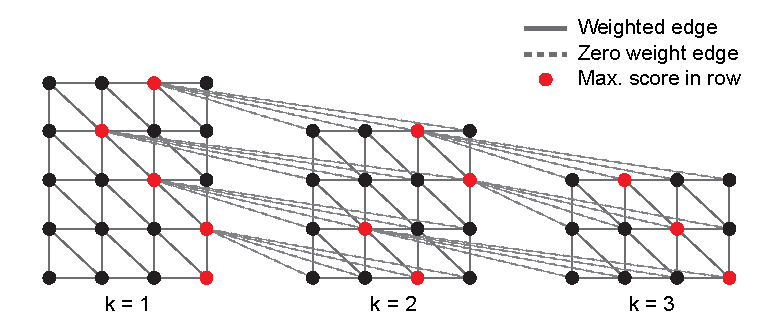
\includegraphics{ch4_fig5.pdf}
\caption[Alignment graph for fragment boundary identification algorithm
  with an arbitrary score function]{
  Alignment graph for fragment boundary identification algorithm
  with an arbitrary score function. The direction of arrows are omitted
  for clarity. The horizontal edges are directed from left to right and
  all other edges are directed from top to bottom.}
\label{frag_alg}
\end{figure}

% Disadvantages
Although this algorithm provides the exact solution to determine optimal
fragment boundaries for each $k$, it has several limitations for use
with real SMURF-seq reads in practice.
% We will usually know the approximate no for frags
As discussed in section \ref{}, when mapping SMURF-seq reads the
approximate mapping locations of fragments would be known after seeding.
Further, if a mapping algorithms performs a preliminary alignment between
parts of the SMURF-seq read and the reference genome, the approximate
fragment boundaries will also be know.
% Needs to start at k=1

% too much time and space
% not banded
% not all parts of the read may be mappable
% repeats


%%%%%%%%%%%%%%%%%%%%%%%%%%%%%%%%%%%%%%%%%%%%%%%%%%%%%%%%%%%%%%%%%%%%%%%%
\subsection{Identifying fragment boundaries in practice}
The initial step in any traditional mapping algorithm is to determine the
approximate mapping locations of the read on the reference genome using
a seeding approach.
%
Some algorithms further generate proto-alignments using the initial
seeds.
For example, BWA-MEM joins seeds that are close to on the read and
reference coordinates and have the same orientation into a ``chain''
\citep{}.
%
Typically, the final step is to perform a Smith-Waterman alignment
between the read and a small region on the reference genome.

% Aligning SMURF-seq reads
Any algorithm to aligning SMURF-seq reads can be expected to have
similar steps. After seeding a SMURF-seq read, seeds from different
fragments on a read would cluster at different locations on the genome,
likely several different location for each fragment due to repeats or
seeding parameters (such as seed length).
%
These seed hits could be further processed to generate preliminary
alignments between parts of the read and the reference genome.
%
Thus, after these steps it is reasonable to assume that approximate
number of fragments and the boundaries of these fragments are known.

%% Final step
The final step of the algorithm would be finalize the number of fragments
and fragment boundaries on a read. For a given number of fragments, the
fragment boundaries can be easily determined such that the alignment
score is maximized (this problem is equivalent to finding a longest path
in a single-source directed acyclic graph).
%
For finding the number of fragments on a SMURF-seq read, for each
fragmentation, we use the
alignment score distribution of random sequences with the same
fragment set to determine the p-value for a fragmentation using the
procedure described in the next section.



%%%%%%%%%%%%%%%%%%%%%%%%%%%%%%%%%%%%%%%%%%%%%%%%%%%%%%%%%%%%%%%%%%%%%%%%
%%%%%%%%%%%%%%%%%%%%%%%%%%%%%%%%%%%%%%%%%%%%%%%%%%%%%%%%%%%%%%%%%%%%%%%%
%%%%%%%%%%%%%%%%%%%%%%%%%%%%%%%%%%%%%%%%%%%%%%%%%%%%%%%%%%%%%%%%%%%%%%%%
\section{Alignment score of a SMURF-seq read}
The alignment score of a SMURF-seq read given by equation \ref{}
is the sum of the alignment score of each of individual fragment
for a particular fragmentation with $k$ fragments,
and algorithms given in section \ref{} determine the best fragmentation
so that the alignment score is maximized.

The alignment score of a SMURF-seq read is a non-decreasing function with
the number of fragments, as the score function does not penalize for
increasing the number of fragments on a read. Thus, a SMURF-seq read
aligned with $k$ fragments can always be aligned with $k+1$ with a
score at least as high as with $k$ fragments.

As an example of how the alignment score of a SMURF-seq read grows as a
function of $k$, consider a read consisting of $f$ fragments (typically
$>$ 20 for a SMURF-seq read), however, $f$ is not known \emph{a priori}.
% one fragment
If the read is aligned to the reference genome as one fragment, it is
likely going to be aligned to a random location on the reference genome;
Alternatively, one of the fragments in the read could align close to its
true location, and the flanking fragments would align to flanking
regions on the genome (essentially aligning fragments to a random
location on the genome for these flanking fragments).
% two fragments
Similarly, if the read is aligned as two fragments, it is likely going
to align to two random location on the genome, or at most two fragments
could align to regions close to their true location. With the alignment
score with two fragments at least as high as with one fragment.
% 3 to f-1
As the read is aligned with increasing $k$ up to $f-1$, the number of
the number of bases on a read that are aligned to its true location on
the genome will increase, and number of based aligned to random location
would decrease. Although there will always bases that are not mapped to
its true location.
% f fragments
At $k=f$ all the fragments on the read would be mapped to their true
locations with no bases aligned to random locations.
% beyond f
As $k$ increased beyond $f$, each fragment will be split into shorter
fragments, the fragmentation location likely being at locations of
sequencing errors (with a small increase in the alignment score). And if
there are no more sequencing errors, the split can be anywhere on the
read, with the alignment score remaining the same.
% m fragments
At $k=m$, i.e. each base on the read aligns as one fragment with the
highest possible alignment score.

\begin{figure}[t!]
\centering
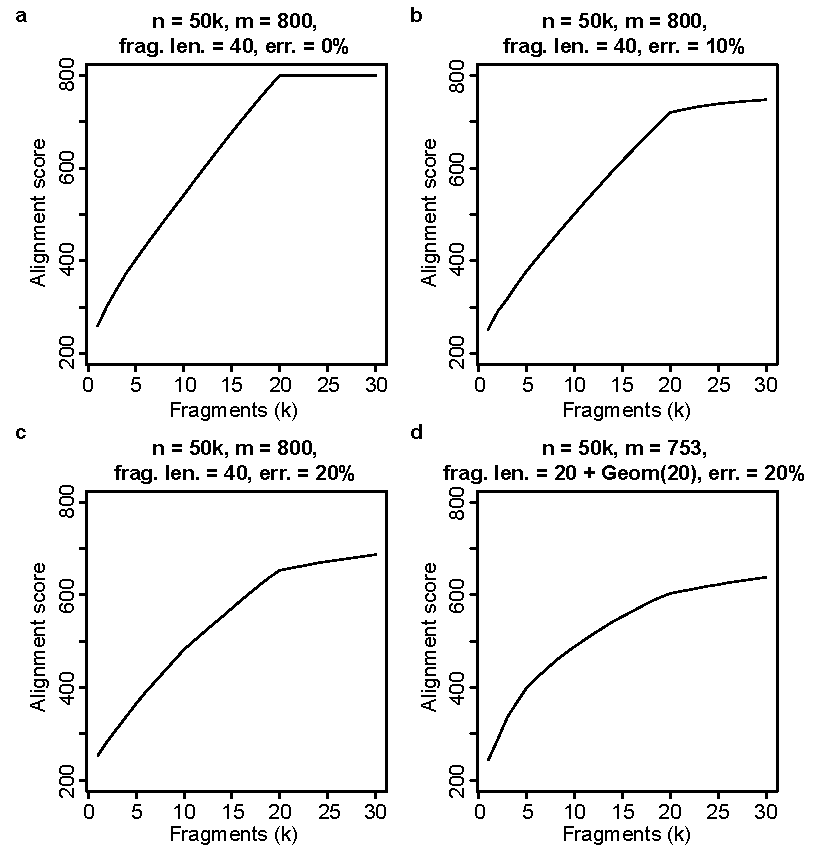
\includegraphics{aln_score.pdf}
\caption[Alignment score of SMURF-seq read as a function of number of
  fragments]{
  Alignment score of SMURF-seq read as a function of number of
  fragments.
  (a) Alignment score of a SMURF-seq read with 20 fragment (40 bp each)
  that does not have any errors.
  (b) Alignment score with 10\% errors.
  (c) Alignment score with 20\% errors.
  (d) Alignment score of a read with 20 fragments generated from $20 +
  \text{Geom}(20)$ distribution and with 20\% errors.}
\label{aln_score}
\end{figure}

% alignment score with no sequencing errors
Consider a simulated SMURF-seq read from a genome of length 50 kb, the
read has 20 fragments each of length 40 bp, and the read does not have
any sequencing errors. Fig.~\ref{aln_score}a shows the alignment score
as a function of the number of fragments $k$, with scoring a match as
1, a mismatch as 0, and not allowing indels. At $k=1$, the score is at
the lowest, and increases with $k$. At $k=20$ every fragment is mapped
to it true location, and since the read does not have any sequencing
errors, the score is equal to the read length. For $k > 20$, the score
remains at the maximum.

% alignment score with sequencing errors
When a SMURF-seq read has sequencing errors, the alignment score
increases with the number of fragments, but would not reach the peak at
$k=20$ (Fig~\ref{aln_score}b; read similar to \ref{aln_score}a, but with
10\% mismatch errors). The alignment score continues to increase beyond
$k=20$ but at a lower rate, and would eventually equal the read length
as the number of fragments increase. Similarly, Fig.~\ref{aln_score}c
ducts the alignment score for a read with 20\% mismatch errors. However,
the due to higher errors, the score is lower at $k=20$, and the curve
``flattens''.

% align score with errors and random fragment lengths
For a real SMURF-seq read, the fragment lengths cannot expected to be
constant. Fig.~\ref{aln_score}d shows the score of of read with 20
fragments, with each fragment of lengths sampled from a $20 +
\text{Geom}(20)$ (mean fragment length of 40 bp) distribution. The
alignment score has increase, but the change in slope at $k=20$ is not
prominent.

%%%%%%%%%%%%%%%%%%%%%%%%%%%%%%%%%%%%%%%%%%%%%%%%%%%%%%%%%%%%%%%%%%%%%%%%
%%%%%%%%%%%%%%%%%%%%%%%%%%%%%%%%%%%%%%%%%%%%%%%%%%%%%%%%%%%%%%%%%%%%%%%%
%%%%%%%%%%%%%%%%%%%%%%%%%%%%%%%%%%%%%%%%%%%%%%%%%%%%%%%%%%%%%%%%%%%%%%%%
\section{Score distribution under a random model}
% Whey do we need this
Calculation of p-value for aligning a SMURF-seq read with a given
fragmentation requires the null distribution of aligning reads
generated at random with the same with the same fragmentation. The
problem of finding the null distribution is defined as:
% Problem definition
consider strings $T$ and $S$ are generated by drawing letters independently
from the same distribution from an alphabet $a \in \Sigma$ with
probability $p_a$ such that $\sum_{a \in \Sigma} p_a = 1$.  For a given
fragment set $P$ containing $k$ elements, we need to determine the
distribution of $score_T(S, P)$.
%% Score function
We use the following score function to obtain the distribution of
$score_T(S,k)$:
\begin{equation*}
\label{exact_score}
score(a,b)=\begin{cases} 1 & \text{if } a = b \\
            0 & \text{if } a\neq b \\
            -\infty & \text{otherwise.}
\end{cases}
\end{equation*}

% Summary of what follows
To determine the distribution of $score_T(S, P)$, we first consider the score
distribution when $k = 1$, i.e. the entire read aligns as one fragment.
Then, we consider the score distribution when $k > 1$ as the sum of $k =
1$ distributions. We also empirically show that the form of the null
distribution when using a generalized scoring function is similar to the
distribution obtained with score function defined above.

%%%%%%%%%%%%%%%%%%%%%%%%%%%%%%%%%%%%%%%%%%%%%%%%%%%%%%%%%%%%%%%%%%%%%%%%
\subsection{Score distribution of one fragment}
%% How fragment identification problem differs from these
The score distribution of $score_T(S,1)$ has similarities to the score
distribution of local alignment \citep{} and profile alignment \citep{},
but also differs from these.  The distribution of $score_T(S,1)$ differs
from the local alignment as we require an end-to-end alignment of $S$ to
a substring of $T$, and also differs from the profile score distribution
since the letters of $S$ are generated at random.
%% distribution for k = 1
Based on these results, the distribution of $score_T(S,1)$ is likely to
follow an extreme value distribution.

\begin{figure}[t!]
\centering
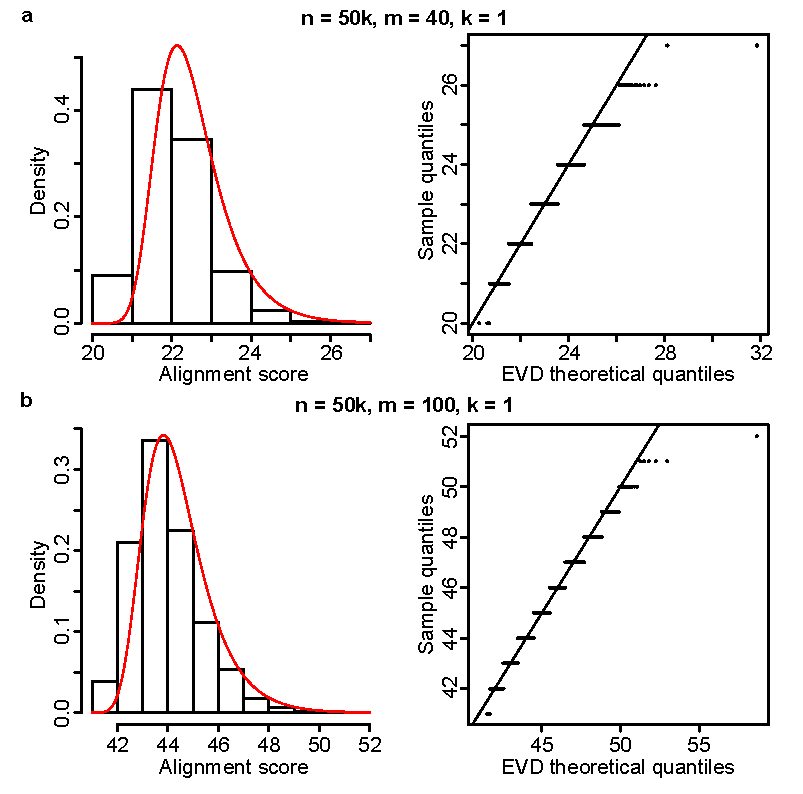
\includegraphics{k1_evd.pdf}
\caption[Extreme value distribution approximation for $score_T(S,1)$]{
  Extreme value approximation for $score_T(S,1)$.
  Empirical score distribution of $score_T(S,1)$ with a fitted
  EVD using the method of moments estimator.
  Q-Q plot comparing the theoretical and empirical distributions are shown.
  (a) $m=40$.
  (b) $m=100$.}
\label{evd_approx}
\end{figure}

% heuristic of proof
Let $X_j$ denote the score of aligning $S$ with $T[j \dots j+m-1]$, then
\[X_j = \sum_{i=0}^{m-1} score(S[i],T[j+i]), j = 0, \dots, n-m+1.\]
Since the letters of T and S are iid, we have \[X_j \sim binom(m,p)\]
where $p = \sum_{a=\Sigma} p_a^2$.  For a large enough $m$, $X_j$ can
be approximated by a normal distribution as \[X_j \sim N(mp, mp(1-p)).
\] $score_T(S,1)$ is the maximum score over all positions in $T$,
\[score_T(S,1) = \max_{0 \leq j \leq n-m+1} X_j.\] $score_T(S,1)$ is a
maximum of normal distributions, which follows an extreme value
distribution (EVD) \citep{kotz2000extreme}.
%% m-dependence
Here, we have a dependence between $X_j$ and $X_k$ for $|j - k| < m$.

%% distribution and qq plot
We verified score distribution of $score_T(S,1)$ by generating a random
genome of length 50kb from the DNA alphabet with equal probabilities,
and reads of length 40 bp and 100 bp. For each read length, we
determined the score distribution by aligning 10,000 reads generated at
random (Fig.~\ref{evd_approx}a, b). The parameters for the EVD was
estimated using the method of moments.
%% Distribution as a function of fragment length
Further, the score distribution for increasing read lengths shows an
increasing trend in the mean and standard deviation of the distribution
(Fig.~\ref{evd_approx}c, d).

\begin{figure}[t!]
\centering
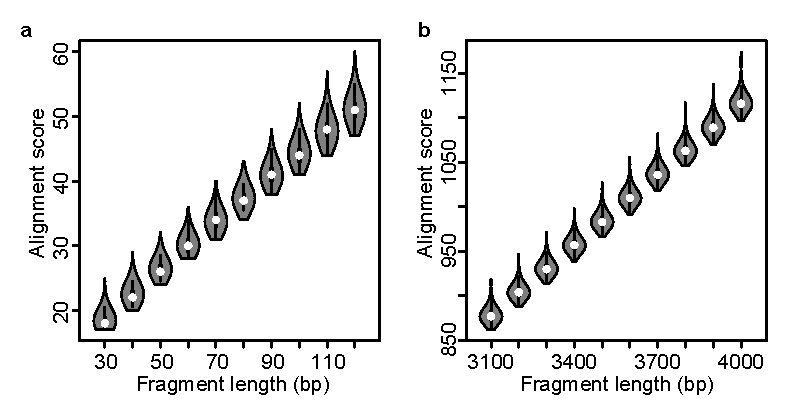
\includegraphics{k1_empirical.pdf}
\caption[Empirical score distribution for $score_T(S,1)$]{
  Empirical score distribution approximation for $score_T(S,1)$.
  (a) Empirical score distribution for $m$ corresponding to shorter
  fragments.
  (b) Empirical score distribution form $m$ corresponding to longer
  fragments.}
\label{evd_empirical}
\end{figure}


%%%%%%%%%%%%%%%%%%%%%%%%%%%%%%%%%%%%%%%%%%%%%%%%%%%%%%%%%%%%%%%%%%%%%%%%
\subsection{Score distribution for a given fragment set}
%% sum of k=1 distributions
The distribution of $score_T(S,k)$ for $k > 1$ and a given $P$ is the
sum of $k$ independent distributions of $score_T(S,1)$, i.e the
distribution of $score_T(S,k)$ is the sum of $k$ independent extreme
value distributions \[score_T(S,k) = \sum_{i=1}^{k} score_T(S[P_i \dots
P_{i+1}], 1).\]
% independence
The independence of the distributions for each fragment is justified
because it is required that $n >> m$, and the probability of two
fragments to aligning to overlapping location on $T$ is extremely small.

\begin{figure}[t!]
\centering
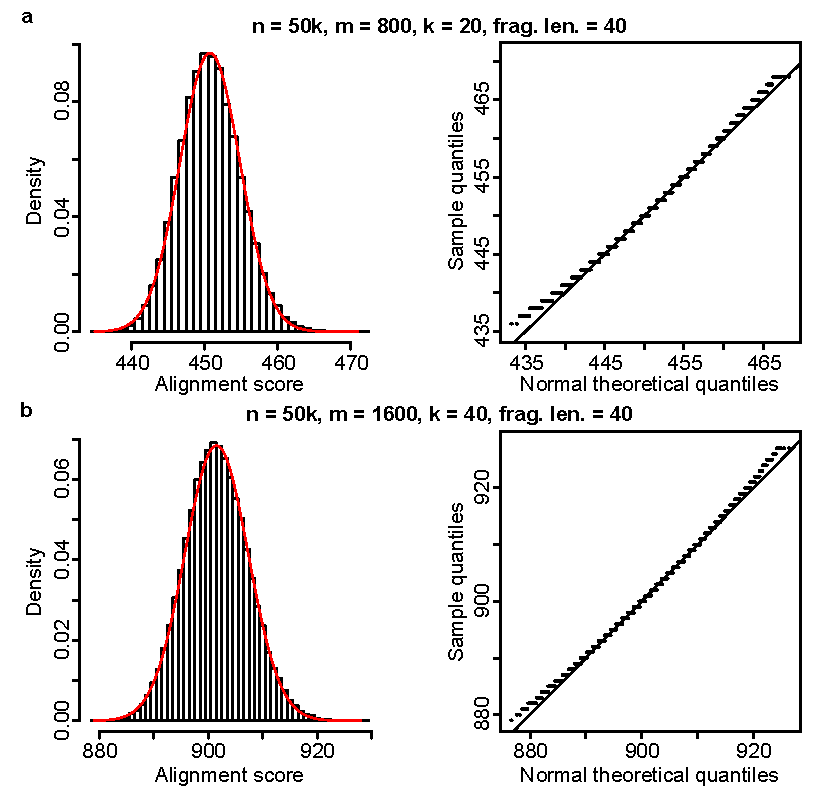
\includegraphics{fl40_norm.pdf}
\caption[Normal approximation for $score_T(S,k)$ with equal fragment
  lengths]{
  Normal approximation for $score_T(S,k)$ with equal fragment lengths.
  Empirical score distribution of $score_T(S,k)$ with a fitted
  normal using the method of moments estimator. All fragments are 40 bp.
  Q-Q plot comparing the theoretical and empirical distributions are shown.
  (a) $m=800, k=20$.
  (b) $m=1600, k=40$.}
\label{norm_const}
\end{figure}

%% Sum of EVDs
The distribution of the sum and linear combination of extreme value
distributions has been studied \citep{cetinkaya2001scalable,
marques2015distribution,loaiciga1999analysis,nadarajah2008exact}.  In
\citep{loaiciga1999analysis} the exact distribution of two independent
Gumbel distributions is given and in \citep{nadarajah2008exact} the exact
distribution of the linear combination of Gumbel distributions is given.
%
However, these distributions do not follow a ``standard'' distribution.

%% Central limit theorem, constant fragment length
Since each the distribution of score of each fragment is independent,
when the fragments are of equal lengths, the distribution of
$score_T(S,k)$ is a sum of i.i.d. random variables. Thus, we can apply
the central limit theorem to approximate the score distribution to a
normal distribution as $k \to \infty$. To test the convergence to
$score_T(S,k)$ to normal, we compared the score distribution to the
normal distribution for $k$ that are typical for a SMURF-seq read
(Fig.~\ref{norm_const}). The fragments lengths for all the comparisons
were kept constant at 40 bp, and the parameters for the normal
distribution was determined using the method of moments estimator.

%% unequal fragment lengths
In aligning a SMURF-seq read, we cannot expect the fragment lengths to
be equal. The distribution of $score_T(S,k)$, when the fragment lengths
differ, is a sum of independent, but not identical, random variables. We
empirically verified that this distribution converges to normal
(Fig.~\ref{norm_geom}). For each $k$, the fragment lengths were
generated from at random from a geometric distribution.

\begin{figure}[t!]
\centering
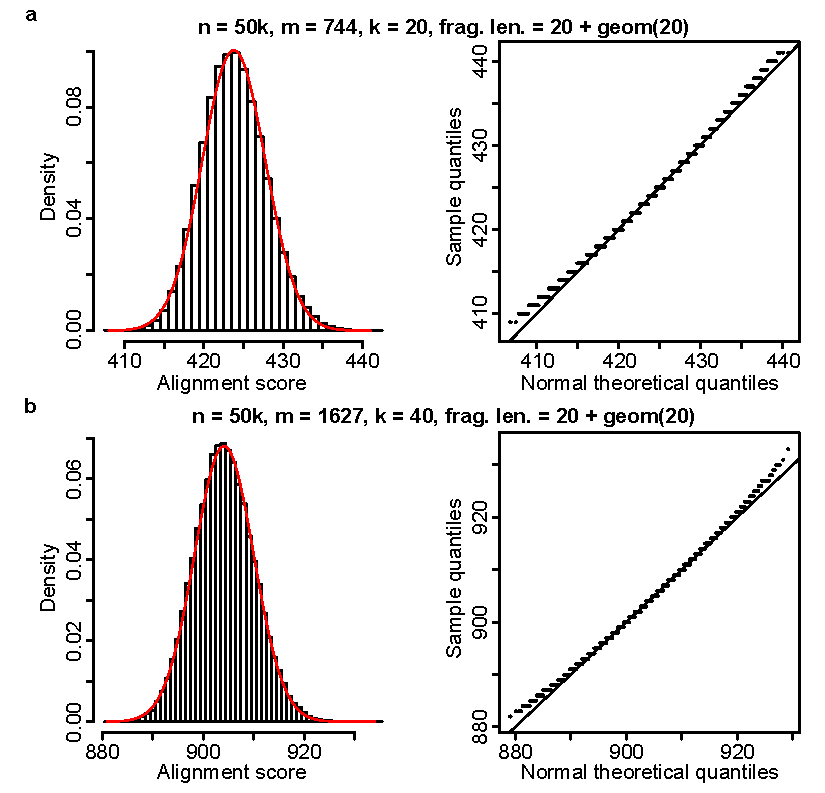
\includegraphics{geom_fl_norm.pdf}
\caption[Normal approximation for $score_T(S,k)$ with random fragment
  lengths]{
  Normal approximation for $score_T(S,k)$ with random fragment lengths.
  Empirical score distribution of $score_T(S,k)$ with a fitted
  normal using the method of moments estimator. The fragment lengths are
  generated from a geometric distribution with mean 100. Q-Q plot comparing
  the theoretical and empirical distributions are shown.
  (a) $m=2188, k=20$.
  (b) $m=3332, k=40$.}
\label{norm_geom}
\end{figure}


%%%%%%%%%%%%%%%%%%%%%%%%%%%%%%%%%%%%%%%%%%%%%%%%%%%%%%%%%%%%%%%%%%%%%%%%
%%%%%%%%%%%%%%%%%%%%%%%%%%%%%%%%%%%%%%%%%%%%%%%%%%%%%%%%%%%%%%%%%%%%%%%%
%%%%%%%%%%%%%%%%%%%%%%%%%%%%%%%%%%%%%%%%%%%%%%%%%%%%%%%%%%%%%%%%%%%%%%%%
\section{Estimating the optimal fragment set}
%% Algorithm
The score distribution of aligning a random read $S_\mathrm{rand}$ to a
random genome $T_\mathrm{rand}$ can be used to estimate the optimal $k$
for aligning a SMURF-seq read $S_\mathrm{SMURF}$ to a reference genome
$T_\mathrm{ref}$.
% Alignm SMURF-seq read
For a SMURF-seq read and, find the
best alignment score $k_\mathrm{score}$ and the fragment set
$k_\mathrm{P}$ for all $k$ from $1$ to $m$ using algorithms given
in section \ref{}. In practice, $k$ can be restricted to a much smaller
subset of possible values, and the goal is to determine a value of $k$
that best represents the fragments that were ligated to generated the
read.
%

As described in the previous section, the null score distribution of
aligning a read generated at random for $k=1$ follows an extreme value
distribution, and a normal distribution for sufficiently large $k$.  For
each $k$, the parameters for the null distributions can be estimated
from the empirical distribution by aligning random reads with the
fragment set $k_\mathrm{P}$.
%
The p-value for each $k$ can be determined by finding the probability of
a score greater than $k_\mathrm{score}$ from the null distribution.
Finally, the optimal $k$ for a read is the one with the lowest p-value
(Algorithm \ref{p_val_alg}).

\begin{algorithm}[H]
\caption{OptimalK $(T,S)$}
\begin{algorithmic}[1]
  \STATE $k_\mathrm{opt} \leftarrow 1$
  \STATE $\Pr_\mathrm{opt} \leftarrow 1$
  \FOR {$k \leftarrow 1$ \TO $m-1$}
    \STATE $k_\mathrm{score}, k_\mathrm{P} \leftarrow
              FragMatch(T_\mathrm{ref},S_\mathrm{SMURF},k)$
    \STATE $k_{\Pr} \leftarrow \Pr(score_{T_\mathrm{rand}}
              (S_\mathrm{rand},k_\mathrm{P}) > k_\mathrm{score})$
    \IF {$k_{\Pr} < \Pr_\mathrm{opt}$}
      \STATE $\Pr_\mathrm{opt} \leftarrow k_{\Pr}$
      \STATE $k_\mathrm{opt} \leftarrow k$
    \ENDIF
  \ENDFOR
  \RETURN $k_\mathrm{opt}$
\end{algorithmic}
\label{p_val_alg}
\end{algorithm}

%% Explanation
As discussed in section \ref{}, as $k$ increases up to $k_\mathrm{opt}$
the number of bases on a SMURF-seq that are aligned to its true location
on the reference genome would increase and the bases aligned to random
locations would decrease. Thus, getting further away from a random
alignment with an expected decrease in p-value. At $k = k_\mathrm{opt}$,
all bases are aligned to their true locations, and would have the lowest
p-value. As $k$ gets farther away from $k_\mathrm{opt}$, fragments on a
read are further split into smaller fragments with a small increase in
alignment score, and eventually with fragment aligning to random
locations on the reference. Thus, getting closer to a random alignment
with an expected increase in p-value.

% Figure for a single read with alignment score, null distribution and
% p-value
\begin{figure}[t!]
\centering
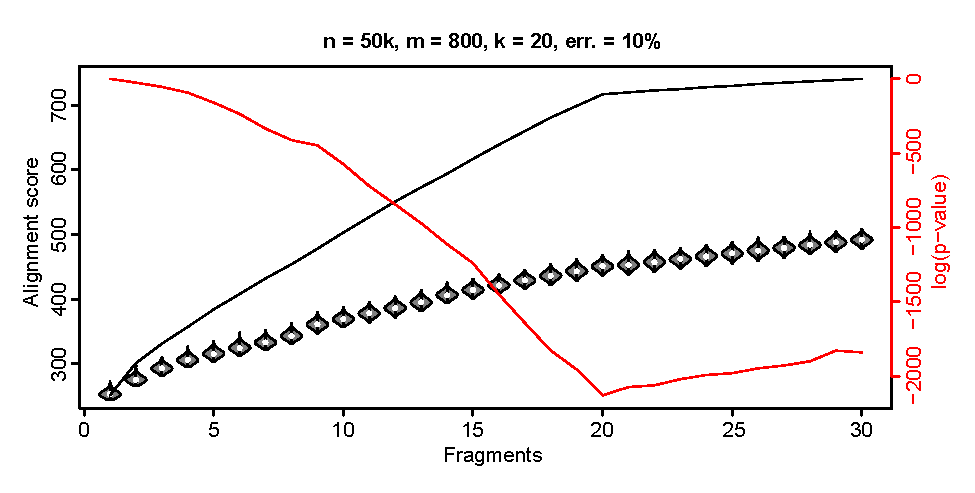
\includegraphics{pval.pdf}
\caption[Determining the optimal fragmentation of a SMURF-seq read]{
  Determining the optimal fragmentation of a SMURF-seq read. The black
  line is the alignment score of a simulated SMURF-seq read with 20
  fragments of 40 bp each, and with 10\% mismatch errors. The violin plots
  are the empirical null distributions using fragment set corresponding
  the best alignment score for each $k$. The red line is the p-value for
  each $k$ determined from the alignment score and the null distribution.
  The optimal fragmentation has the lowest p-value.}
\label{pval_calc}
\end{figure}

%% example
As an example, we simulated a reference genome of length 50 kb with the
DNA alphabet having equal probabilities.
%
A simulated SMURF-seq read with 20 fragments each of length 40 bp was
generated from this genome, and 10\% mismatch sequencing errors was
introduced.
%
This read are then mapped back to the reference genome for values of $k
= 1$ to $30$ using algorithm \ref{} (scoring a match as 1, a mismatch as
0, and not allowing indels), yielding the fragment set that maximizes
the alignment score for each $k$.
%
These fragment sets were then used to generate the null distribution by
simulating a random reference genome with the same base probabilities,
and aligning 10,000 random reads with fragment start locations based on
the fragment set.
%
The p-value for each fragmentation was determined using an EVD for $k=1$
and normal distributions for $k > 1$ with parameters estimated using the
method of moments from the simulated reads (although the normal
approximation does not hold for small values of $k$, we have included it
for clarity).
%
The fragmentation with the smallest p-value was considered as the
optimal fragmentation, and as expected, $k = 20$ has the lowest p-value;
With the p-value increasing on either side of $k = 20$
(Fig.~\ref{pval_calc}).

The example considered here is simplified to illustrate the procedure
to determine the optimal fragmentation of a SMURF-seq read. In aligning
real SMURF-seq reads: (1) The reference genome would be significantly
larger (e.g. the human genome) with different base (or dinucleotide)
probabilities. (2) The fragments lengths cannot expected to be constant.
(3) The sequencing error model will depend on the properties of the
sequencing technology used. (4) The alignment score used would depend on
the sequencing error model and would allow indels (with possibly
different penalties for gap open and gap extend). (5) Parameters for the
null distribution were determined empirically, which cannot be done in
practice. Some of these issues are considered in the following sections.  

%%%%%%%%%%%%%%%%%%%%%%%%%%%%%%%%%%%%%%%%%%%%%%%%%%%%%%%%%%%%%%%%%%%%%%%%
\subsection{Fast computation of p-values}

% Figure comparing the fitted empirical score distribution using the two
% methods

%%%%%%%%%%%%%%%%%%%%%%%%%%%%%%%%%%%%%%%%%%%%%%%%%%%%%%%%%%%%%%%%%%%%%%%%
%%%%%%%%%%%%%%%%%%%%%%%%%%%%%%%%%%%%%%%%%%%%%%%%%%%%%%%%%%%%%%%%%%%%%%%%
%%%%%%%%%%%%%%%%%%%%%%%%%%%%%%%%%%%%%%%%%%%%%%%%%%%%%%%%%%%%%%%%%%%%%%%%
\section{Open problems}





\subsection{Aligning with a general score function}

% negative score for mismatches

% negative score for mismatch and indels



